\documentclass[11pt]{beamer}
\usetheme{JuanLesPins}
\usepackage[utf8]{inputenc}
\usepackage[spanish,es-nodecimaldot]{babel} 
\usepackage{amsmath}
\usepackage{amsfonts}
\usepackage{amssymb}
\usepackage{graphicx}
\usepackage{adjustbox}
\usepackage{array}
\spanishdecimal{.}
\author{M. en E. Sergio Nava}
\title{Probabilidad}
%\setbeamercovered{transparent} 
%\setbeamertemplate{navigation symbols}{} 
%\logo{} 
%\institute{} 
\date{Viernes 28 de septiembre de 2018} 
%\subject{} 


\AtBeginSection[]  % The commands within the following {} will be executed at the start of each section.
{
\begin{frame} % Within each "frame" there will be one or more "slides."  
\frametitle{Contenido} % This is the title of the outline.
\tableofcontents[currentsection]  % This will display the table of contents and highlight the current section.
\end{frame}
} % Do not include the preceding set of commands if you prefer not to have a recurring outline displayed during your presentation.


\begin{document}

\begin{frame}
\titlepage

\end{frame}


%\begin{frame}
%\tableofcontents
%\end{frame}


\begin{frame}
\begin{center}
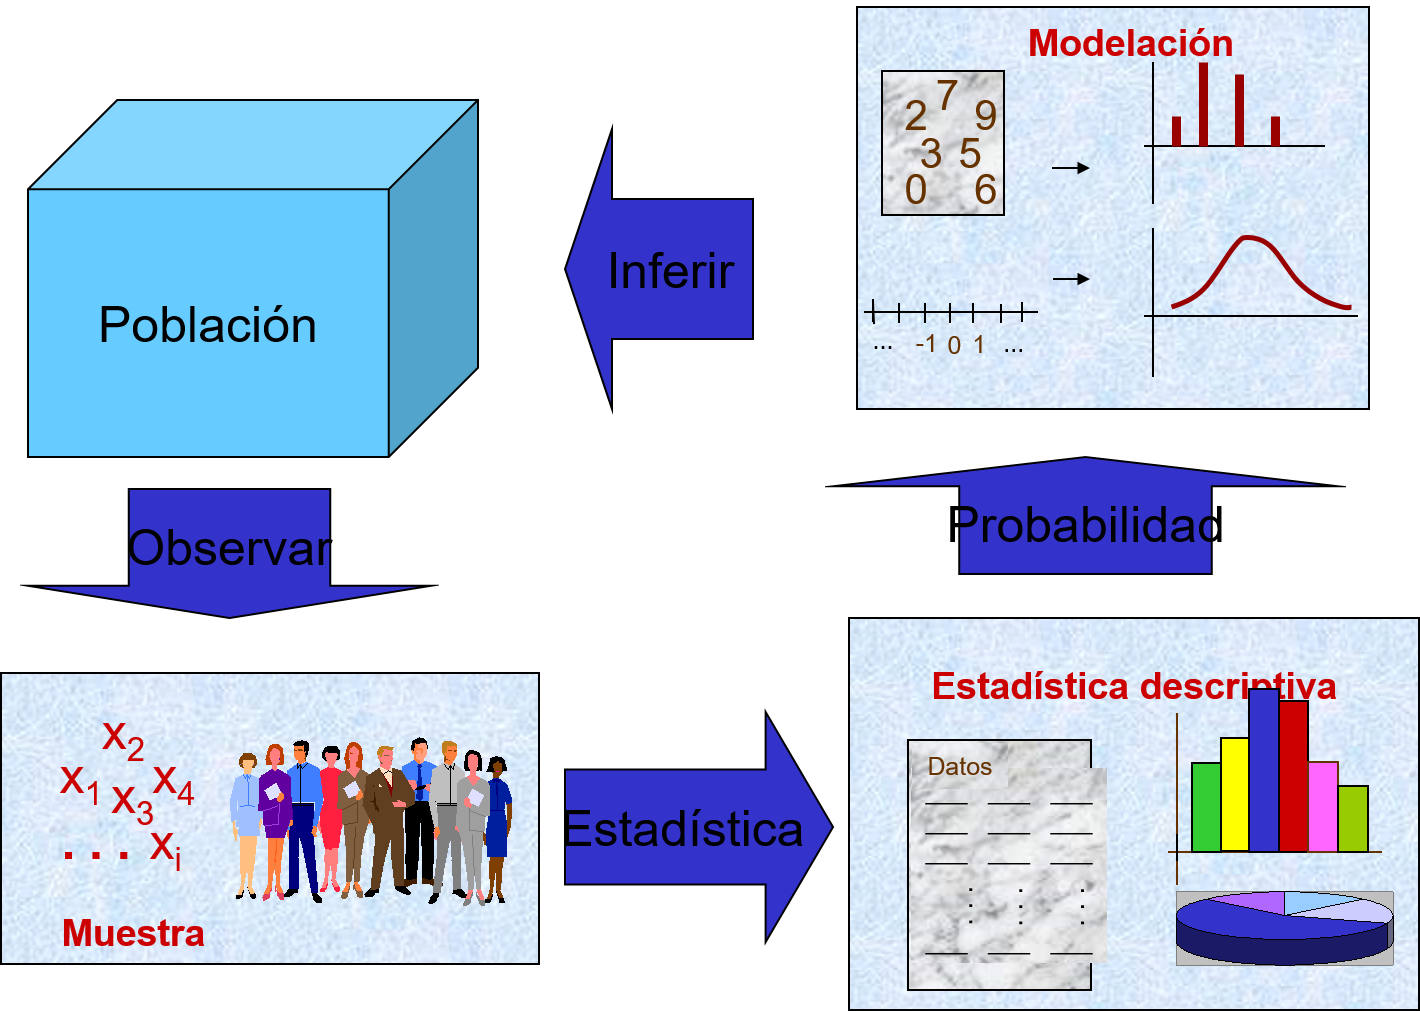
\includegraphics[scale=0.4]{imagenes/primerdiagrama.png} 
%ilustracion41%
\end{center}
\end{frame}



\begin{frame}{Probabilidad}
Un fenómeno es determinista si de antemano se conoce el resultado del mismo, todo lo no determinista es aleatorio. \\ \bigskip

La probabilidad es una medida del conocimiento o desconocimiento que se tiene acerca de un fenómeno no previsible (aleatorio). 
\end{frame}

\section{Experimento aleatorio, espacio muestral, evento} 


\begin{frame}{Experimento (probabilístico o aleatorio)}
\begin{enumerate}
\item Es el proceso por medio del que se registra una observación o medición.

\item Es aquel que proporciona diferentes resultados aun cuando se repite siempre de la misma manera.

\item En particular, para el estudio de la probabilidad nos interesa observar aquellos experimentos cuyo resultado no es pronosticable con certeza, es decir, aquellos en que existe aleatoriedad.
\end{enumerate}
\end{frame}

\begin{frame}{}
\centering
\adjustbox{max height=\dimexpr\textheight-5.5cm\relax,
           max width=\textwidth}{

\begin{tabular}{|l|l|l|}
\hline
\textbf{Experimento} & \textbf{Resultado} \\ \hline
Lanzar una moneda & Sol,águila \\ \hline
Seleccionar una parte mecánica para inspección & Defectuosos, no defectuosos \\ \hline
Telefonema de ventas & Compra, no compra \\ \hline
Tirar un dado & 1, 2, 3, 4, 5, 6 \\ \hline
Jugar un partido de fútbol & Ganar, perder, empatar \\ \hline
\end{tabular}
}
\end{frame}

\begin{frame}{Elemento o punto muestral}
\begin{itemize}
\item Un elemento muestral o punto muestral es un posible resultado de un experimento.
\bigskip
\item Ejemplo: Del experimento de lanzar una moneda, un elemento muestral es SOL, y otro es AGUILA.

\end{itemize}
\end{frame}

\begin{frame}{Espacio muestral}
Es la colección de todos los posibles resultados de un experimento ( o todos los posibles elementos o puntos muestrales).

\bigskip

Normalmente lo denotamos como S.

\begin{center}
	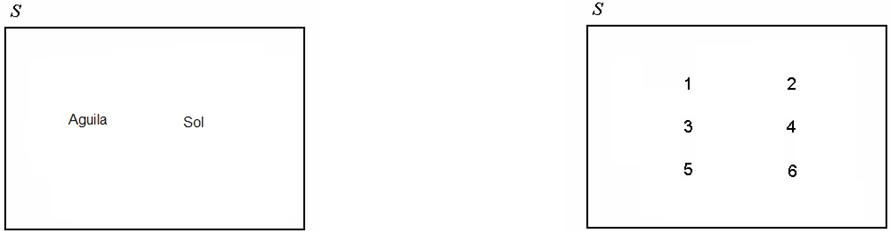
\includegraphics[scale=0.5]{imagenes/prob1.JPG} 
\end{center}

\end{frame}

\begin{frame}{}
\centering
\adjustbox{max height=\dimexpr\textheight-5.5cm\relax,
           max width=\textwidth}{
\begin{tabular}{|l|l|l|}
\hline
\textbf{Experimento} & \textbf{Espacio muestral} \\ \hline
Lanzar una moneda & S=\{Sol,águila\} \\ \hline
Seleccionar una parte para inspecciónarla & S=\{Defectuosos, no defectuosos\} \\ \hline
Telefonema de ventas & S=\{Compra, no compra\} \\ \hline
Tirar un dado & S=\{1, 2, 3, 4, 5, 6\} \\ \hline
Jugar un partido de fútbol & S=\{Ganar, perder, empatar\} \\ \hline
\end{tabular}
}
\end{frame}

\begin{frame}{Evento o Suceso}
\begin{itemize}
\item Un evento es un subconjunto del espacio muestral.
\item Al ser un subconjunto incluye la posibilidad de que esté todo el conjunto (todo el espacio muestral) y que incluya nada (conjunto vacío).
\end{itemize}
\begin{flushright}
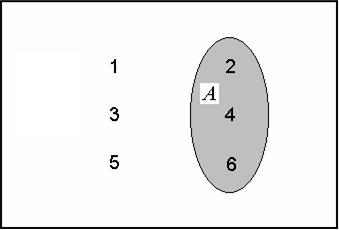
\includegraphics[scale=0.4]{imagenes/prob2.JPG}
\end{flushright}
\end{frame}
 
\begin{frame}{Ejemplo de Evento}
\begin{itemize}

\item “Obtener un número par al lanzar un dado” :
\begin{center}
$A=\lbrace2,4,6\rbrace$
\end{center}
\item “Observar menos de 5 piezas defectuosas en una muestra de 100”: 
\begin{center}
$B=\lbrace0,1,2,3,4\rbrace$
\end{center}
\item “Tener más de 50 llamadas telefónicas en una hora en un conmutador” : 
\begin{center}
$C=\lbrace51,52,...,\infty\rbrace$
\end{center}
\end{itemize}
\begin{flushright}
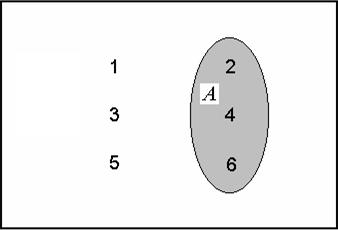
\includegraphics[scale=0.4]{imagenes/prob3.JPG} 
\end{flushright}
\end{frame}


\begin{frame}{Propiedades}
Dados tres sucesos \textit{A, B} y \textit{C} de un espacio muestral \textit{S} 

\begin{align*} 
\mbox{Conmutativa} &: \left\lbrace \begin{array}{l} A\cup B = B \cup A \\ A\cap B = B \cap A \\ \end{array} \right. \\ 
\mbox{Asociativa} &: \left\lbrace \begin{array}{l} A \cup (B \cup C) =(A \cup B) \cup C \\ A \cap (B \cap C) =(A \cap B) \cap C \\ \end{array} \right. \\ 
\mbox{Distributiva} &: \left\lbrace \begin{array}{l} A \cup (B \cap C) =(A \cup B) \cap (A \cup C) \\ A \cap (B \cup C) =(A \cap B) \cup (A \cap C) \\ \end{array} \right. \\ 
\mbox{Leyes de Morgan} &: \left\lbrace \begin{array}{l} \overline{A\cup B} = \overline{A} \cap \overline{B} \\ \overline{A\cap B} = \overline{A} \cup \overline{B} \\ \end{array} \right. 
\end{align*}
\end{frame}

\section{Probabildad}

\begin{frame}{Axiomas de Probabilidad}
Sean \textit{S} cualquier espacio muestral definido y \textit{$E_{i}$} cualquier evento de este, es decir 
\textit{$E_{i} \subset S$}

	Se llamará función de probabilidad a \textit{$P(E_{i})$} si satisface los siguientes axiomas:
\begin{enumerate}

\item $0\leq P(E_{i})\leq  1$
\item $P(S)= 1$
\item Para dos eventos $E_{1}$ y $E_{2}$ con $E_{1} \cap E_{2}= \emptyset$, $P(E_{1} \cup E_{2})= P(E_{1})+ P(E_{2})$

\end{enumerate}

\end{frame}
\begin{frame}{Problema Fundamental}
\begin{itemize}
\item Dado un espacio muestral discreto con resultados $E_{1}, E_{2}, ... , E_{n}$, el experimento aleatorio queda caracterizado si asignamos un valor $P(E_{i})$ no negativo a cada resultado $E_{i}$ que verifique
\begin{center}
$P(E_{1})+ P(E_{2})+ \cdots + P(E_{n})=1$
\end{center}
\item Ejemplo. Se lanza dos veces una moneda.
\begin{center}
$\lbrace XX,XC,CX,CC \rbrace$
\end{center}


	Se asigna probabilidad $1\diagup 4$ a cada uno de los cuatro resultados.
	
¿ Es una asignación correcta?

\end{itemize}
\end{frame}

\begin{frame}{Complemento de un evento}
Dado un evento A, el {\it complemento} de A se define como el conjunto formado por todos los puntos muéstrales que {\it no están} en A. El complemento se denota como $A^{c}$ , $A^{\prime} $ ó $\Bar{A}$.

$$P(A)+P(A^{c})=1 $$
\\Por lo tanto:
$$P(A^{c})=1-P(A)$$

\begin{flushright}
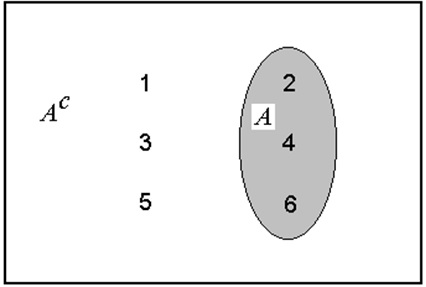
\includegraphics[scale=0.4]{imagenes/prob4.jpg} 
\end{flushright}

\end{frame}
\begin{frame}{Implicaciones de los axiomas}
\begin{itemize}
\item Para cualquier evento $E$, $P(E^{c})=1-P(E)$

\bigskip 
\item $P(\emptyset)=0$

\bigskip 
\item Si el evento $E_{1}$ esta contenido en el evento $E_{2}$, entonces $P(E_{1})\leq P(E_{2})$
\end{itemize}
\end{frame}

\begin{frame}{Unión de dos eventos}
\begin{itemize}
\item La unión de A y B es el evento que contiene todos los puntos muestrales que pertenecen a A o a B, o a ambos.
\item La unión de A y B se representa con 
$A \cup B$
\end{itemize}
\begin{center}
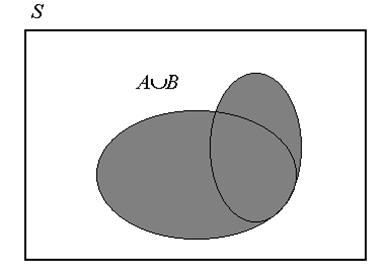
\includegraphics[scale=0.4]{imagenes/prob5.JPG} 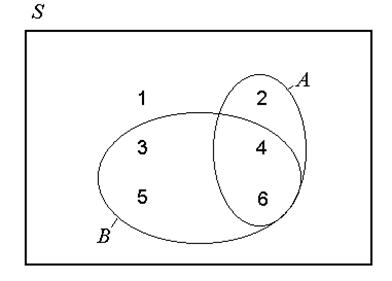
\includegraphics[scale=0.4]{imagenes/prob6.JPG} 
\end{center}
\end{frame}

\begin{frame}{Intersección de dos eventos}
Dados dos eventos, A y B, la intersección de A y B es el evento que contiene los puntos muestrales que pertenecen simultáneamente a A y a B, y se representa como $A \cap B$.
\begin{center}
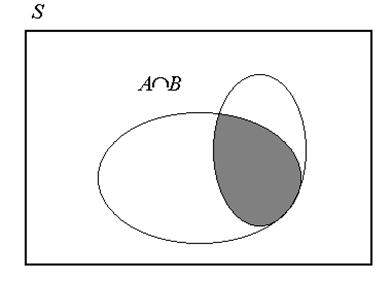
\includegraphics[scale=0.4]{imagenes/prob7.JPG} 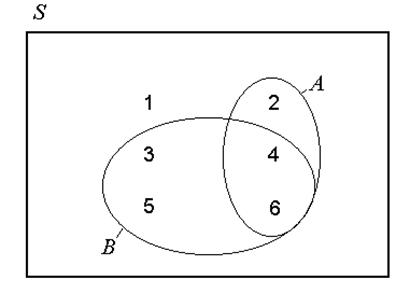
\includegraphics[scale=0.4]{imagenes/prob8.JPG}  
\end{center}
\end{frame}

\begin{frame}{Ley aditiva}
La ley aditiva es útil cuando se tienen dos eventos y se quiere conocer la probabilidad de al menos uno de 
ellos.

\bigskip $P(A \cup B)=P(A)+P(B)-P(A \cap B)$

\begin{center}
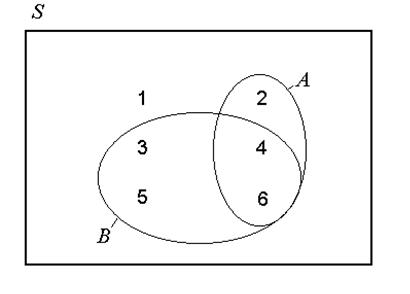
\includegraphics[scale=0.4]{imagenes/prob9.JPG} 
\end{center}
 $P(A \cup B)=P(A)+P(B)-P(A \cap B)$\\ $P(A \cup B)=3/6+4/6-2/6=5/6$
\end{frame}

\begin{frame}{Eventos mutuamente excluyentes (ajenos)}
Se dice que dos eventos son mutuamente excluyentes (ajenos) si no tienen puntos muestrales  en común.
\begin{center}
 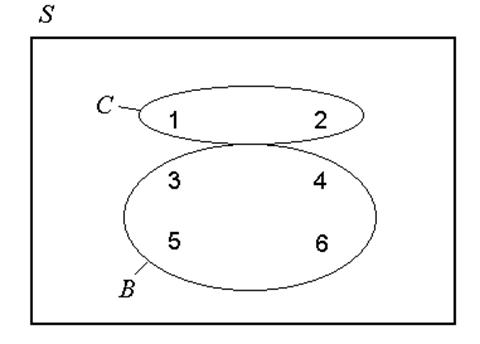
\includegraphics[scale=0.4]{imagenes/prob10.JPG}
 \end{center} 
\end{frame}

\begin{frame}{Eventos mutuamente excluyentes}
Si los eventos B y C son mutuamente excluyentes entonces 
\begin{center}
$B \cap C= \emptyset$
\end{center}

\bigskip entonces
\begin{center}
$P(B\cap C)=P(\emptyset)=0$
\end{center}

\bigskip por lo tanto
\begin{center}
$P(B \cup C)=P(B)+P(C)$
\end{center}
\end{frame}

\section{Probabilidad Condicional}
\begin{frame}{Probabilidad condicional}
\begin{itemize}
\item Supongamos que nos interesa un evento B con probabilidad P(B).
\item Si obtenemos nueva información y vemos que ha ocurrido un evento relacionado, representado por A, quisiéramos aprovechar esta información para calcular la probabilidad de B. Esa nueva probabilidad se representa por $P(B \mid A)$ y significa la probabilidad de que ocurra el evento B dado que A ya ocurrió.
\end{itemize}
\end{frame}

\begin{frame}{Probabilidad condicional}
\begin{center}
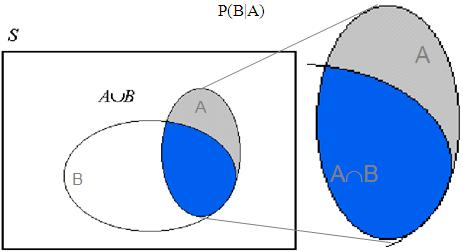
\includegraphics[scale=0.7]{imagenes/prob12.JPG} 
\end{center}
\end{frame}

\begin{frame}{Probabilidad condicional}
$P(B \mid A)=P(A \cap B)/P(A)$

\bigskip Esta es la probabilidad condicional de un evento B dado un evento A.

$P(B \mid A)=(2/6)/(3/6)=2/3$
\begin{center}
 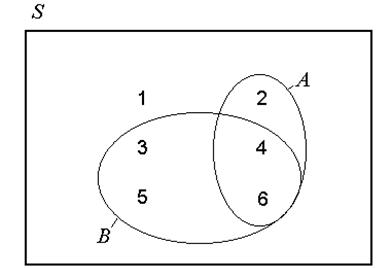
\includegraphics[scale=0.4]{imagenes/prob13.JPG} 
\end{center}
\end{frame}

\begin{frame}{Regla de multiplicar}
$P(A \cap B)=P(B \mid A)P(A)=P(A \mid B)P(B)$

\bigskip $P(A \cap B)=(2/3)(1/2)=(2/6)$

\bigskip $P(A \cap B)=(2/4)(2/3)=(4/12)=(2/6)$
\begin{flushright}
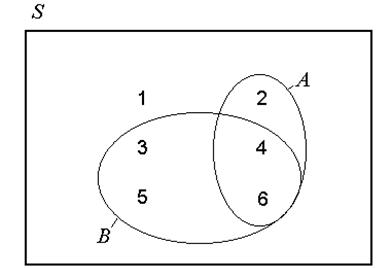
\includegraphics[scale=0.4]{imagenes/prob13.JPG} 
\end{flushright}
\end{frame}

\begin{frame}{Intuir  la probabilidad condicionada}
\begin{center}
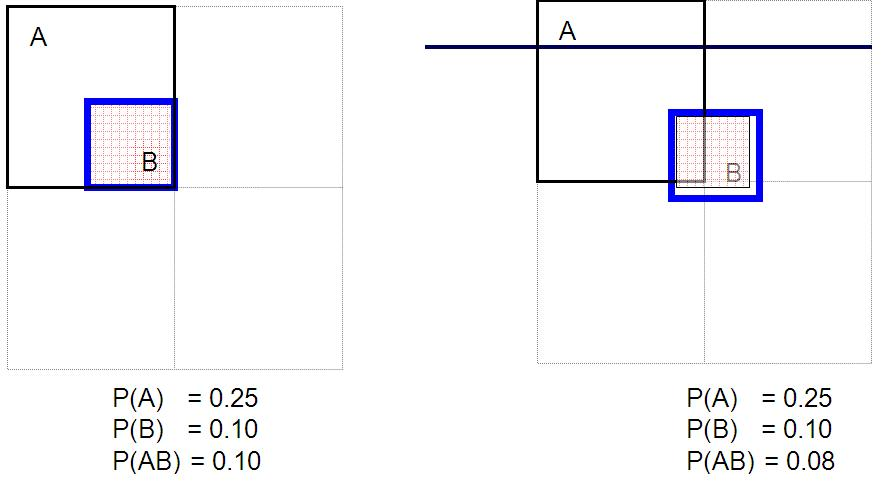
\includegraphics[scale=0.4]{imagenes/prob14.JPG} 
\end{center}
\begin{center}
¿Probabilidad de A sabiendo que ha pasado B?


$P(A \mid B)=1 \hspace{45pt} P(A \mid B)=0.8$
\end{center}
\end{frame}
\begin{frame}{Intuir  la probabilidad condicionada}
\begin{center}
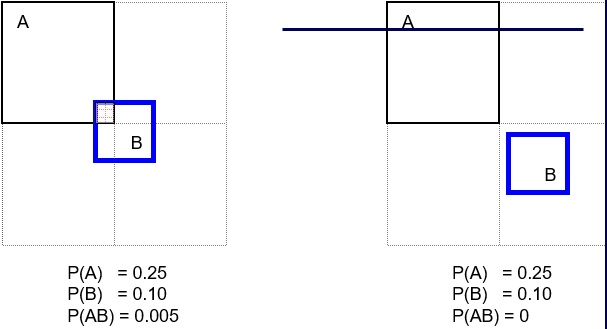
\includegraphics[scale=0.4]{imagenes/prob15.jpg} 
\end{center}
\begin{center}
¿Probabilidad de A sabiendo que ha pasado B?
\end{center}
\begin{center}
$P(A \mid B)=0.05  \hspace{45pt} P(A \mid B)=0$
\end{center}
\end{frame}
\begin{frame}{Ejemplo de Urna: 2 Negras y 3 Blancas}
Se extraen dos bolas al azar, una detrás de otra, ¿cuál es la probabilidad de que una sea Blanca y la otra Negra?
\bigskip 
\bigskip 
\begin{center}
\begin{tabular}{ll}
Sin reemplazo & {\scriptsize $P(B1 \cap N2)= P(B1)P(N2 \mid B1)= (3/5)(2/4)=3/10$}  \\
 & \\
 & \\
 Con reemplazo & {\scriptsize $P(B1 \cap N2)= P(B1)P(N2 \mid B1)= (3/5)(2/5)=6/25$}  \\ 
\end{tabular}
\end{center}
\end{frame}
\begin{frame}{Ejemplo Osteoporosis}
\textbf{EJEMPLO:} En una muestra de $1000$ individuos elegidos al azar, entre una población de enfermos de osteoporosis $760$ eran mujeres.
\bigskip 
\begin{itemize}

\item ¿Qué porcentaje de mujeres hay en la muestra? \\ $760/1000=0.76=76\%$

\item Si elegimos a un individuo de la población, qué probabilidad hay de que sea mujer:
\\ La noción frecuentista de probabilidad nos permite aproximarlo a $P(Mujer)=0.76$


\item ¿Cuál es la probabilidad de que elegido un individuo de la población sea hombre:
\\ $P(Hombre)=P(Mujer^\prime)=1-0.76=0.24$
\end{itemize}

\end{frame}
\begin{frame}{Cont. Ejemplo osteoporosis}
Se sabe de otros estudios que entre los individuos con osteoporosis, aprox. la cuarta parte de las mujeres fuman y la tercera parte de los hombres. Elegimos a un individuo al azar de la población de enfermos.
\begin{itemize}
\item ¿Qué probabilidad hay de que sea mujer fumadora?
\begin{equation*}
\begin{split}
P(Mujer \cap Fumar) & = P(Mujer) P(Fumar \mid Mujer) \\
& =  0.76 x \frac{1}{4} = 0.19
\end{split}
\end{equation*}
\item ¿Qué probabilidad hay de que sea un hombre fumador?
\begin{equation*}
\begin{split}
P(Hombre \cap Fumar) & = P(Hombre) P(Fumar \mid Hombre)\\
& = 0.24 x \frac{1}{3} = 0.08
\end{split}
\end{equation*}
\end{itemize}

\end{frame}

\section{Independencia Estadística}
\begin{frame}{Independencia}
Si el conocimiento de la ocurrencia de un suceso B cambia la probabilidad de que ocurra otro A, se dice que A y B son \textbf{dependientes}, en ese caso $P(A \mid B) \neq P(A)$.
  
 \bigskip 
  
  
Cuando el suceso A es \textbf{independiente} de B, la ocurrencia de B no cambia la probabilidad de A, es decir $P(A \mid B) = P(A)$. Ni la ocurrencia de A cambia la probabilidad de B, es decir $P(B \mid A) = P(B)$.

\end{frame}
\begin{frame}{Independencia}
Se dice que dos eventos son independientes si, y sólo si, cualquiera de las siguientes proposiciones es verdadera.
\begin{enumerate}
\item $P(A \mid B)= P(A)$
\item $P(B \mid A)= P(B)$
\item $P(A \cap B)= P(A)P(B)$
\end{enumerate}
\end{frame}
\begin{frame}{Independencia en nuestro ejemplo}
\begin{enumerate}
\item $P(A \mid B)= P(A)= \frac{1}{2}$
\bigskip 
\item $P(B \mid A)= P(B)= \frac{2}{3}$
\bigskip 
\item $P(A \cap B)= P(A)P(B)= (\frac{1}{2})( \frac{2}{3}) =\frac{1}{3}$
\end{enumerate}
\bigskip 
Entonces A y B son independientes
\begin{flushright}
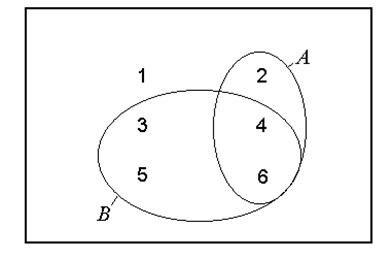
\includegraphics[scale=0.3]{imagenes/prob16.jpg} 
\end{flushright}
\end{frame}

\begin{frame}{Independencia (3 o más sucesos)}
Tres sucesos A,B y C son independientes si
\begin{itemize}
\item $P(A \cap B \cap C)=P(A)P(B)P(C)$
\item $P(A \cap B)=P(A)P(B)$
\item $P(A \cap C)=P(A)P(C)$
\item $P(B \cap C)=P(B)P(C)$
\end{itemize}
\bigskip
Los sucesos $A_{1}$,$A_{2}$,...,$A_{n}$ son idependientes si cualquier subconjunto $A_{i1}$,$A_{i2}$,...,$A_{ik}$ cumple
\begin{itemize}
\item $P(A_{i1} \cap A_{i2} \cap ...  \cap A_{ik})=P(A_{i1})P(A_{i2}) \cdots P(A_{ik})$
\end{itemize}
\end{frame}
\section{* Métodos para asignar probabilidad}
\begin{frame}{Métodos para asignar probabilidad}
\begin{enumerate}
\item Método clásico (laplace): Equiprobabilidad 
\bigskip
\item Método de la frecuencia relativa (Von Mises, 1931) 
\bigskip
\item Método subjetivo
\end{enumerate}
\end{frame}

\begin{frame}{Método clásico (equiprobables)}
Sea un experimento con un número finito de resultados excluyentes y equiprobables, la probabilidad del evento A es \\ \bigskip 
\begin{center}
$P(A)=\frac{N(A)}{N}$
\end{center}
donde N es el número de resultados posibles del experimento y N(A) el número de resultados favorables al evento A.

\end{frame}
\begin{frame}{Ejemplos (equiprobables)}
\begin{itemize}
\item Lanzar una moneda. $S={C,X}$
\begin{center}
$P(X)=\frac{1}{2}$
\end{center}
\item Lanzar un dado. $S={1,2,3,4,5,6}$
\begin{center}
$P(\mbox{``Número par''})=\frac{3}{6}=\frac{1}{2}$
\end{center}
\item Jugar a la lotería
\bigskip
\item Juegar al melate
\end{itemize}
\end{frame}
\begin{frame}{Lanzamiento de dos dados}
\begin{center}
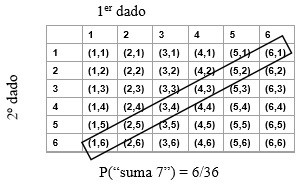
\includegraphics[scale=0.9]{imagenes/prob17.jpg} 
\end{center}
\end{frame}
\begin{frame}{Ejemplo de Urna: 2 Negras y 3 Blancas}
\begin{flushright}
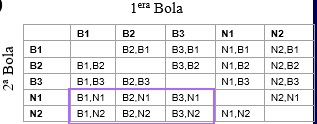
\includegraphics[scale=0.6]{imagenes/prob18.jpg} 
\end{flushright}
Se extraen dos bolas al azar, una detrás de otra, sin reposición (es decir sin reemplazo).
 \begin{center}
 $P(\text{`}1^{a}\text{ Blanca y }2^{a}\text{ Negra'})=\frac{6}{20}=\frac{3}{10}$
 \end{center}

\end{frame}
\begin{frame}{Ejemplo de Urna: 2 Negras y 3 Blancas}
\begin{flushright}
 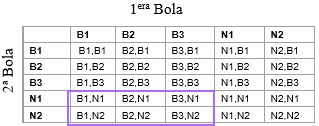
\includegraphics[scale=0.6]{imagenes/prob19.jpg}
 \end{flushright} 
Se extraen dos bolas al azar, una detrás de otra, con reposición (es decir con reemplazo).
\begin{center}
$P(\text{`}1^{a}\text{ Blanca y }2^{a}\text{ Negra'})=\frac{6}{25}$
\end{center}

\end{frame}
\begin{frame}{Combinatoria: 5 objetos tomados de dos en dos}
\begin{center}
 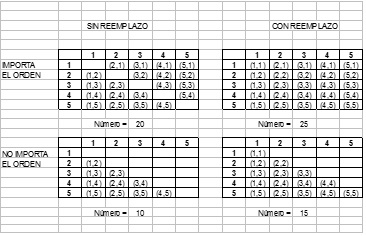
\includegraphics[scale=1]{imagenes/prob20.jpg}
 \end{center} 
\end{frame}
\begin{frame}{Combinatoria: Número posible de reordenaciones de $n$ objetos tomados de $r$ en $r$}
\begin{center}
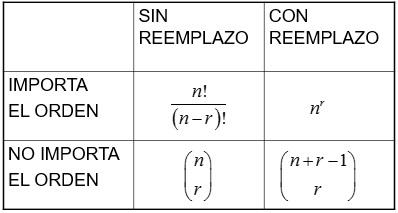
\includegraphics[scale=0.8]{imagenes/prob21.jpg} 
\end{center}

\end{frame}
\begin{frame}{Ejemplo Melate}
\begin{itemize}
\item ¿Cuantos posibles resultados hay en el juego del Melate? \\(Consideremos que son 44 números y se seleccionan seis de ellos).
\bigskip
\item ¿Cual es la probabilidad de acertar a los 6 números ganadores?
\end{itemize}
\end{frame}

\begin{frame}{melate}
\begin{center}
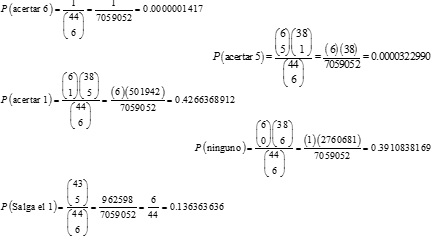
\includegraphics[scale=0.9]{imagenes/prob22.jpg} 
\end{center}
\end{frame}
\begin{frame}{melate}
\begin{center}
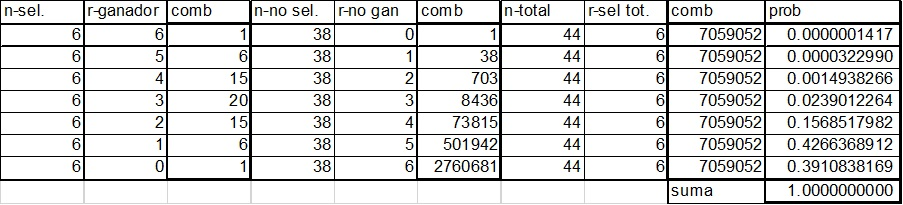
\includegraphics[scale=0.45]{imagenes/prob23.jpg} 
\end{center}
\end{frame}
\begin{frame}{Cumpleaños}
Probabilidad de que en un grupo de r=25 personas haya al menos dos con el mismo cumpleaños
\begin{center}
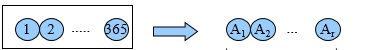
\includegraphics[scale=0.8]{imagenes/prob24.jpg} 
\end{center}
$A=$"No haya ninguna coincidencia"

\bigskip
$P(A)=\dfrac{365x(365-1)x...x(365-r+1)}{365^{r}}$

\bigskip
$P(\overline{A})=1-P(A),\hspace{20pt}R=25\rightarrow P(\overline{A})=0.578$

\end{frame}
\begin{frame}
\begin{Large}
\begin{flushleft}
\textbf{Métodos de asignar probabilidades (Sección opcional)}
\end{flushleft}
\end{Large}

\end{frame}

\begin{frame}{Método de la frecuencia relativa}
La probabilidad $P(A)$ de un evento $A$ es el límite
\begin{center}
$P(A)= \lim_{n\rightarrow \infty }\cfrac{n_{A}}{n}$
\end{center}
donde $n_A$ es el número de veces que ha ocurrido $A$ al repetir el experimento $n$ veces en idénticas condiciones.
\\ El método consiste en asignarle a la probabilidad de que ocurra un evento, la frecuencia relativa de dicho evento.
\begin{center}
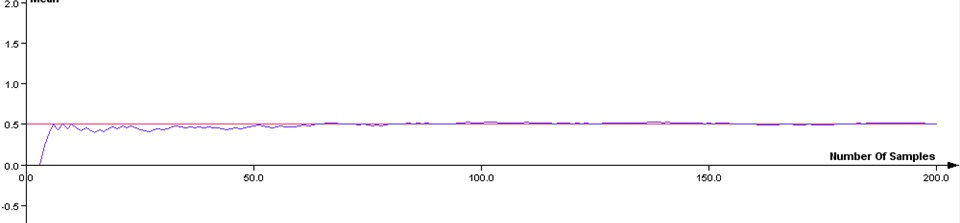
\includegraphics[scale=0.5]{imagenes/prob25.jpg} \\Número de caras/Número de lanzamientos
\end{center}
\end{frame}
\begin{frame}{En 540 sorteos de melate de 634 al 1180}
\begin{center}
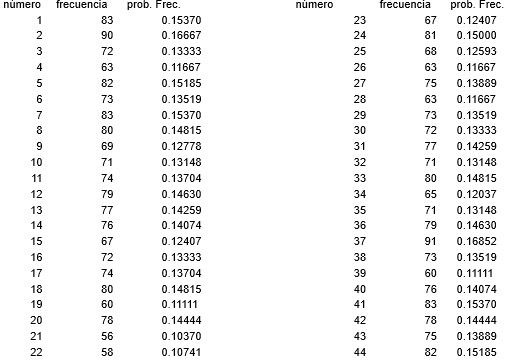
\includegraphics[scale=0.7]{imagenes/prob26.jpg} 
\end{center}
\end{frame}
\begin{frame}{Método subjetivo}
\begin{itemize}
\item Asignar a un valor numérico al grado de creencia que se presente cierto resultado experimental.
\bigskip
\item Ejemplo:
\begin{itemize}
\item ¿Cuál es la probabilidad de que las {\it Chivas} ganen (empaten o pierdan) el próximo partido?.
\item ¿Cuál es la probabilidad de que el caballo {\it sultanito} gane la carrera del próximo domingo?
\end{itemize}
\end{itemize}
\end{frame}
\begin{frame}{Juego}
El juego es el siguiente:
\begin{enumerate}
\item ustedes escogen un número entero del uno al seis, 
\item yo tiro tres dados,  
\begin{itemize}
\item si sale 1, 2 o tres veces el número que escogieron, les pago un dólar, 
\item si no sale ni una vez, ustedes me pagan un dólar.
\end{itemize}
\end{enumerate}
\begin{center}
   ¿Cuál es la probabilidad de que ustedes ganen?
\end{center}
\end{frame}

\section{Probabilidad Total}
\begin{frame}{Sistema exhaustivo y excluyente de sucesos}
Son una colección de sucesos

\begin{center}
$A_{1}, A_{2}, A_{3}, A_{4}, \ldots$
\end{center}
Tales que la unión de todos ellos forman el espacio muestral, y son disjuntos (o mutuamente excluyentes).
\begin{center}
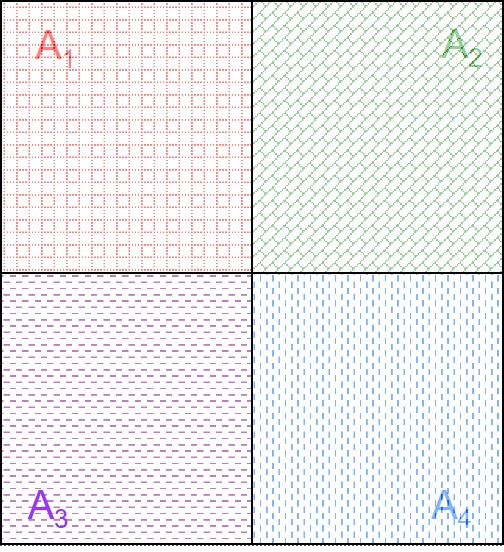
\includegraphics[scale=0.4]{imagenes/prob27.jpg} 
\end{center}
\end{frame}
\begin{frame}{Divide y vencerás}
Todo suceso (evento) $B$, se puede descomponer usando dicho sistema. 
$$B=(B \cap A_{1})\cup (B \cap A_{2})\cup B \cap A_{3})\cup (B \cap A_{4})$$
\begin{center}
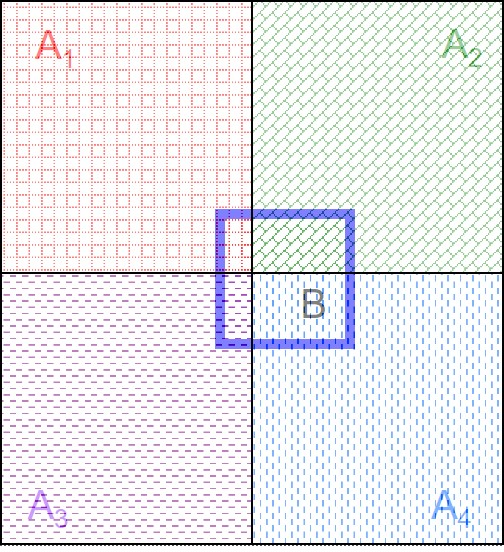
\includegraphics[scale=0.4]{imagenes/prob28.jpg} 
\end{center}
Nos permite descomponer el problema $B$ en {\bf subproblemas más simples}.
\end{frame}
\begin{frame}{Teorema de la probabilidad total}
Si conocemos la probabilidad de $B$ en cada uno de los componentes de un sistema exhaustivo y excluyente de sucesos, entonces podemos calcular la probabilidad de B.
\begin{center}
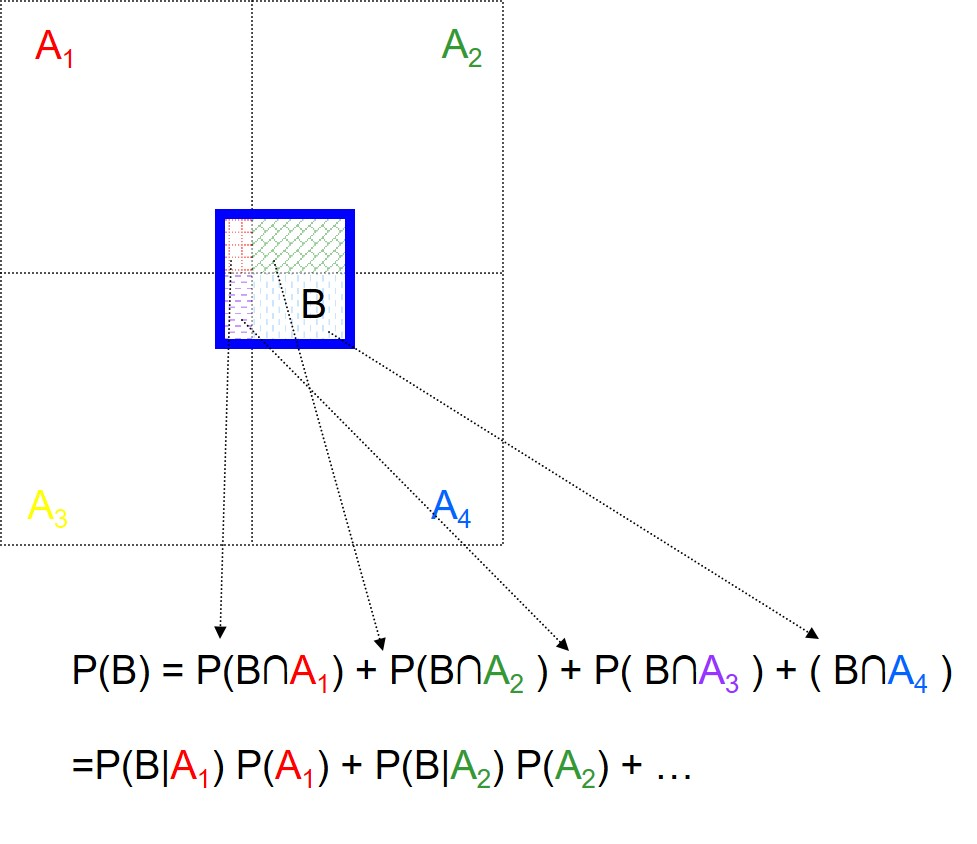
\includegraphics[scale=0.4]{imagenes/prob29.jpg} 
\end{center}
\end{frame}
\begin{frame}{Ejemplo}
En un aula el $70\%$ de los alumnos son mujeres. De ellas el $10\%$ son fumadoras. De los varones, son fumadores el $20\%$.¿Qué porcentaje de fumadores hay en total?

\begin{center}
\begin{tabular}{ll}
 $P(F)=P(F \cap H)+P(F \cap M)$ & 
{\bf T. Probabilidad Total}  \\  
 $=P(F \mid H) P(H)+ P(F \mid M)P(M)$ & Hombres y mujeres forman \\  
 $=0.2x0.3+0.1x0.7$ & un sistema Exh. y Excl.\\  
 $=0.13=13\%$ &  de eventos \\ 
\end{tabular}
\end{center}
\end{frame}

\begin{frame}{Ejemplo (cont.) }
Se elije a un individuo al azar y resulta fumador. ¿Cuál es la probabilidad de que sea un hombre?
\begin{center}

\begin{eqnarray*}
P(H \mid F)&=&P(F \cap H)/P(F) \\
&=&P(F \mid H)P(H)/P(F)\\
&=&0.2x0.3/0.13\\
&=& 0.46=46\% 
\end{eqnarray*}
 \\
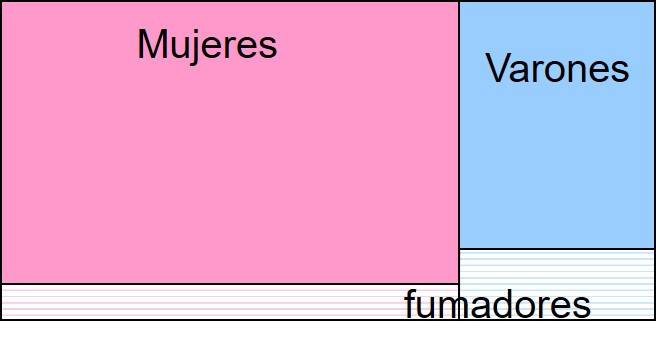
\includegraphics[scale=0.4]{imagenes/prob31.jpg} 
\end{center}
\end{frame}

\begin{frame}{Expresión del problema en forma de arbol}
\begin{center}
$P(F)=0.7x0.1+0.3x0.2=0.13$
\end{center}
\begin{center}
$P(H \mid F)=0.3X0.2/P(F)=0.06/0.13=0.46$
\end{center}
-Los caminos a través de nodos representan intersecciones.


-Las bifurcaciones representan uniones disjuntas.
\begin{center}
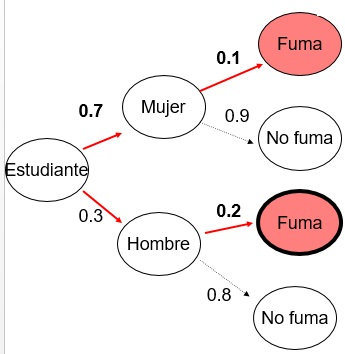
\includegraphics[scale=0.4]{imagenes/prob32.jpg} 
\end{center}
\end{frame}

\section{Regla de Bayes}
\begin{frame}{Teorema de Bayes}
Sea $B_{1}$, $B_{2}$, ... , $B_{n}$ una partición del espacio S tal que $P(B_{j})>0$ para $j=1,2,...,n$ y sea A cualquier suceso con $P(A)>0$, entonces para cualquier $B_{j}$:
\begin{center}
$P(B_{i} \mid A)=\dfrac{P(A \mid B_{i})P(B_{i})}{
\sum_{j=1}^{n}P(A \mid B_{j})P(B_{j})}$
\end{center}

\end{frame}
\begin{frame}{Ejemplo (Bayes)}
\begin{center}
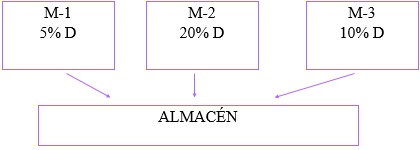
\includegraphics[scale=0.7]{imagenes/prob33.jpg} 
\end{center}
El porcentaje de piezas defectuosas fabricadas por tres máquinas es $5\%$, $20\%$ y $10\%$. La primera fabrica 200 piezas por hora y las otras dos 100 piezas por hora. Todas las piezas  fabricadas  se llevan al almacén. Al final del día se toma una pieza del almacén y es defectuosa, ¿cuál es la probabilidad de que proceda de M-1?

\end{frame}
\begin{frame}{}
\begin{small}
\begin{center}
$P(M_{1} \mid D )= \dfrac{P(D \mid M_{1})P(M_{1})}{P(D \mid M_{1})P(M_{1})+P(D \mid M_{2})P(M_{2})+P(D \mid M_{3})P(M_{3})}$
\end{center}
\begin{center}
$=\dfrac{0.05x0.5}{0.05x0.5+0.20x0.25+0.10x0.25}=0.25$
\end{center}
\begin{center}
$P(M_{2} \mid D )= \dfrac{P(D \mid M_{2})P(M_{2})}{P(D \mid M_{1})P(M_{1})+P(D \mid M_{2})P(M_{2})+P(D \mid M_{3})P(M_{3})}
$
\end{center}
\begin{center}
$=\dfrac{0.20x0.25}{0.05x0.5+0.20x0.25+0.10x0.25}=0.50$
\end{center}

\begin{center}
$P(M_{3} \mid D )= \dfrac{P(D \mid M_{3})P(M_{3})}{P(D \mid M_{1})P(M_{1})+P(D \mid M_{2})P(M_{2})+P(D \mid M_{3})P(M_{3})}
$
\end{center}
\begin{center}
$=\dfrac{0.10x0.25}{0.05x0.5+0.20x0.25+0.10x0.25}=0.25$
\end{center}
\begin{center}
$P(M_{1} \mid D )+P(M_{2} \mid D )+P(M_{3} \mid D )=1$
\end{center}
\end{small}
\end{frame}
\begin{frame}{}
\begin{center}
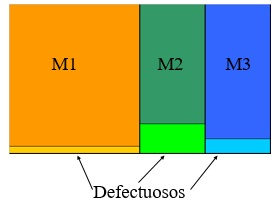
\includegraphics[scale=0.8]{imagenes/prob34.jpg} 
\end{center}
\end{frame}
\begin{frame}{Pruebas diagnósticas}
\begin{footnotesize}
Una {\it prueba diagnóstica} sirve para ayudar a mejorar una estimación de la probabilidad de que un individuo presente una enfermedad.
\begin{itemize}
\item En pricipio tenemos una {\it idea subjetiva} de  $P(Enfermo)$. Nos ayudamos de… 
\begin{itemize}
\item {\bf Incidencia}: Porcentaje de nuevos casos de la  enfermedad en la población.
\item {\bf Prevalencia}: Porcentaje de la población que presenta una enfermedad.
\end{itemize}
\item Por otra parte, para confirmar, usamos una prueba diagnóstica. La misma ha sido evaluada con anterioridad sobre dos grupos de individuos: sanos y enfermos. Así {\it de modo frecuentista} se ha estimado:
\begin{itemize}
\item {\bf Sensibilidad} (verdaderos +)= Tasa de acierto sobre enfermos.
\item {\bf Especificidad} (verdaderos -)= Tasa de acierto sobre sanos.
\end{itemize}
\item A partir de lo anterior y usando el {\it Teorema de Bayes}, podemos calcular las probabilidades a posteriori (en función de los resultados del test): {\bf Índices predictivos}
\begin{itemize}
\item $P(Enfermo \mid Test +) =$ Índice predictivo positivo
\item $P(Sano \mid Test -) =$ {\bf Índice predictivo negativo}
\end{itemize}
\end{itemize}
\end{footnotesize}

\end{frame}
\begin{frame}{Pruebas diagnósticas: aplicación T. Bayes. }
\begin{center}
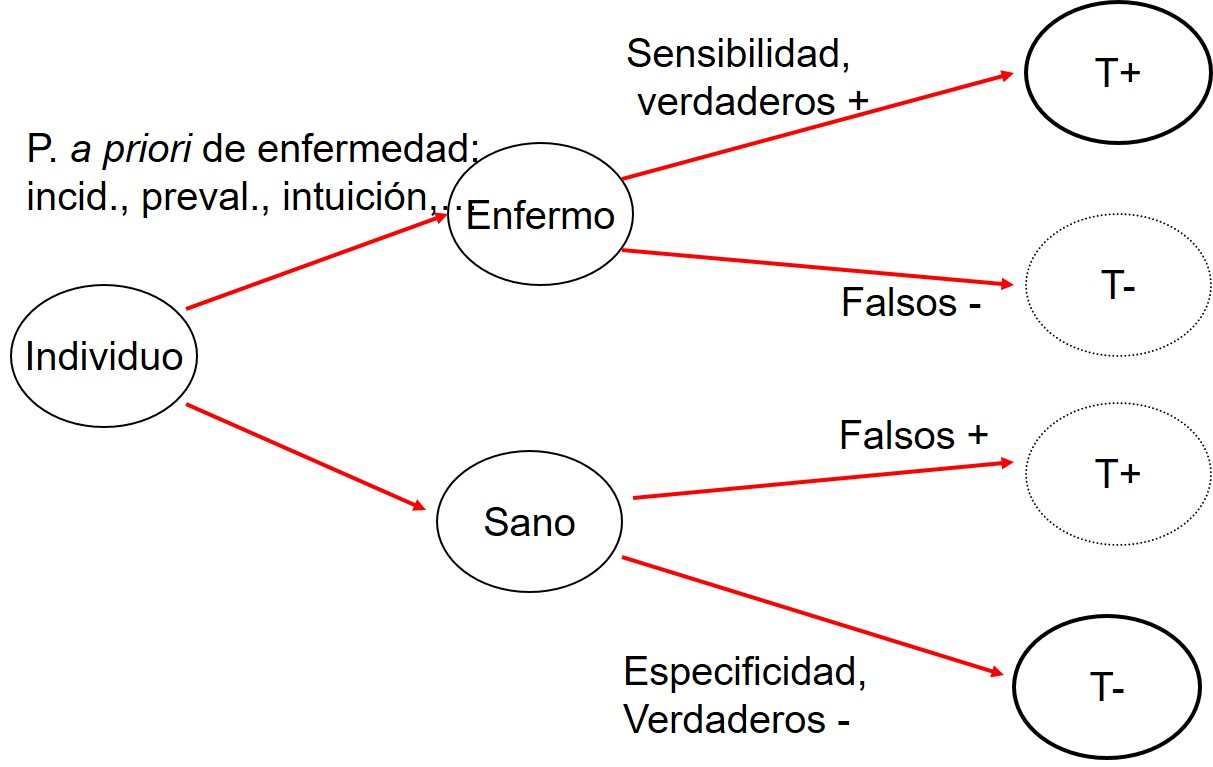
\includegraphics[scale=0.4]{imagenes/prob35.jpg} 
\end{center}
\end{frame}
\begin{frame}{Ejemplo: Pruebas diagnóstica y T. Bayes}
La diabetes afecta al 20 de los individuos que acuden a una consulta. La presencia de glucosuria se usa como indicador de diabetes. Su sensibilidad es de $0.3$ y la especificidad de $0.99$. Calcular los índices predictivos.
 \begin{columns}
    \begin{column}{.6\textwidth}
    \begin{footnotesize}
     \begin{eqnarray*}
P(\textit{Enf} \mid T+)&=&\dfrac{P(\textit{Enf} \cap T+)}{P(\textit{Enf} \cap T+)+P(\textit{Sano} \cap T+)} \\
&=&\dfrac{0.2 \times 0.3}{0.2 \times 0.3+0.8 \times 0.01}=0.88 \\
P(\textit{Sano} \mid T-)&=&\dfrac{P(\textit{Sano} \cap T-)}{P(\textit{Sano} \cap T-)+P(\textit{Enf} \cap T-)}\\
&=&\dfrac{0.8 \times 0.99}{0.8 \times 0.99+0.2 \times 0.7}=0.85
     \end{eqnarray*}
     \end{footnotesize}
    \end{column}
    \begin{column}{.4\textwidth}
    \vspace{0cm}
        \begin{figure}[h]
        \only { 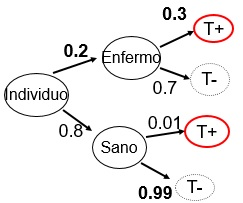
\includegraphics[scale = 0.5]{imagenes/prob36.jpg} }
        \end{figure}
    \end{column}
  \end{columns}
\end{frame}

\begin{frame}{Observaciones}
\begin{footnotesize}
\begin{tabular}{m{15em} m{15em}}
\hline
 En el ejemplo anterior, al llegar un individuo a la consulta tenemos una idea {\it a priori} sobre la probabilidad de que tenga una enfermedad. &  ¿Qué probabilidad tengo de estar enfermo? \\ \hline
A continuación se le pasa una prueba diagnóstica que nos aportará nueva información: Presenta glucosuria o no.   & En principio un $20\%$. Le haremos unas pruebas.\\
\hline En función del resultado tenemos una nueva idea (a posteriori) sobre la probabilidad de que esté enfermo.
\begin{itemize}
\item Nuestra opinión a priori ha sido modificada por el resultado de un experimento. 
\item Relaciónalo con el método científico. 
 \end{itemize}
 &

 Presenta glucosuria. La probabilidad ahora es del $88\%$.\\
\hline
\end{tabular}
\end{footnotesize}
\end{frame}

\begin{frame}{Ejemplo Virus}
Si una persona es portadora del virus A, un análisis de sangre lo detecta el 99\% de las veces. Sin embargo, el test también proporciona “falsos positivos”, indicando la presencia del virus en el 3\% de personas sanas. Si sólo 5 de cada 1000 personas tienen el virus, ¿cuál es la probabilidad de que una persona tenga el virus realmente si el análisis ha dado positivo? \\
\bigskip
\begin{tabular}{ll}
V=$"$Tener el virus$"$ & 
S= $"$El análisis es positivo$"$
\bigskip
\end{tabular}

\begin{center}
\begin{small}
$P(V \mid S)=\dfrac{P(V \cap S)}{P(S)}=\dfrac{P(S \mid V)P(V)}{P(S \mid V)P(V)+P(S \mid \overline{V})P(\overline{V})}$
\end{small}
{\small $=\dfrac{0.99 \times 0.005}{0.99 \times 0.005+0.03 \times 0.995}=0.142$}
\end{center}
\end{frame}
\begin{frame}{Pruebas diagnósticas: aplicación T. Bayes.}
\begin{center}
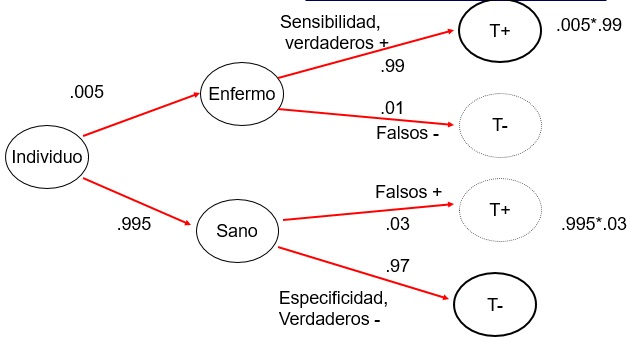
\includegraphics[scale=0.7]{imagenes/prob37.jpg} 
\end{center}

\end{frame}
\begin{frame}{Ejemplo Virus (Aplicado a 1,000,000 personas)}
\begin{tabular}{|l|r|r|r|}
\hline
 & Positivos $S$ & Negativos $\overline{S}$ &Total  \\ \hline
Enfermos $V$ & 4,950 & 50 & 5,000  \\ \hline
Sanos $\overline{V}$  & 29,850 & 96,5150 & 995,000 \\ \hline
Total & 34,800 & 965,200 & 1`000,000 \\ \hline 
\end{tabular} \\
\bigskip
Entre los 34,800 que han dado positivo, sólo 4,950 tienen el virus
\begin{center}
$P(V \mid S)=4,950/34,800=0.142$
\end{center}
\end{frame}
\begin{frame}{Monty hall}
\textit{Supón que estás en un concurso, y se te ofrece escoger entre tres puertas: detrás de una de ellas hay un coche, y detrás de las otras, cabras. Escoges una puerta, digamos la nº1, y el presentador, que sabe lo que hay detrás de las puertas, abre otra, digamos la nº3, que contiene una cabra. Entonces te pregunta: "¿No prefieres escoger la nº2?". ¿Es mejor para ti cambiar tu elección?} 
\end{frame}
\begin{frame}{Monty hall El enunciado completo }
Se ofrece un concurso cuya mecánica es la siguiente:
\begin{itemize}
\item Al concursante se le ofrece la posibilidad de escoger entre tres puertas. Tras una de ellas se encuentra un coche, y tras las otras dos hay una cabra. El concursante gana el premio que se oculta detrás de la puerta que escoja.
\item Después de que el concursante escoja una puerta, el presentador abre una de las otras dos puertas, mostrando una cabra. Siempre puede hacerlo ya que incluso si el concursante ha escogido una cabra, queda otra entre las puertas que ha descartado.
\item Entonces, ofrece al concursante la posibilidad de cambiar su elección inicial y escoger la otra puerta que descartó originalmente, que continúa cerrada. 
\end{itemize}
\bigskip
La pregunta oportuna es: ¿debe hacerlo o no?

\end{frame}
\begin{frame}{Monty hall  Suposiciones iniciales}
Esta solución se basa en tres suposiciones básicas:
\begin{enumerate}
\item que el presentador siempre abre una puerta, 
\item que la escoge entre las restantes después de que el concursante escoja la suya,
\item y que tras ella siempre hay una cabra.
\end{enumerate}
\bigskip Estas suposiciones no se encuentran explícitamente en el enunciado.
\end{frame}

\end{document}

